\documentclass[pdftex,12pt,letter]{article}
\usepackage[margin=0.75in]{geometry}
\usepackage{verbatim}
\usepackage{graphicx}
\usepackage[pdftex,pdfpagelabels,bookmarks,hyperindex,hyperfigures]{hyperref}


%\usepackage{amssymb}
%\usepackage{xspace}

\usepackage{lineno}

\newcommand{\pd}{protoDUNE\ }

\title{Design of the Data Management System for the \pd Experiment}
\date{\today}
\author{M. Potekhin$^a$, B. Viren$^a$, S. Fuess$^b$, O. Gutsche$^b$, R. Illingworth$^b$,\\M. Mengel$^b$,
 A. Norman$^b$\\
\ \\
$^a$\textit{Brookhaven National Laboratory, Upton NY}\\
$^b$\textit{Fermi National Accelerator Laboratory, Batavia IL}}


\begin{document}
\maketitle



\begin{abstract}
The \pd experimental program is designed to test and validate the technologies and design that will be applied to the construction
of the DUNE Far Detector at the Sanford Underground Research Facility (SURF).  The \pd detectors will be run in a dedicated beam line
at the CERN SPS accelerator complex. The rate and volume of data produced by these detectors will be substantial and will require
extensive system design and integration effort. We present a design option based on existing and successful technology developed at
FNAL, the F-FTS.
\end{abstract}
\newpage
\tableofcontents
%\linenumbers
\newpage
%% main text
\section{The \pd Program}
\label{S:1}
\subsection{The Prototypes}
The \pd program will help validate various DUNE technology aspects before proceeding with the construction of the principal DUNE detectors at SURF.
It is designed for measurements with a test beam provided by a dedicated target and beamline system at the CERN SPS accelerator complex.
It also has the potential to be an important platform for realistic Liquid Argon Time Projection Chamber (LArTPC) detector characterization
(e.g. PID, shower response, etc.) utilizing controlled conditions of a test-beam experimental setup. The name ``\pd'' currently applies to two
full-scale LArTPC prototypes based on two different technologies --- single-phase and dual-phase TPCs.
The ``full-scale'' designation is used to describe the fact that the prototypes
contain important (and large) structural and readout elements built according to the specifications (including the size)
of the eventual full detector.

The ``single-phase''  LArTPC functions without amplification in the medium (liquid Argon) and is in essence a very large ionization chamber
equipped with a large number of readout electrodes (wires), each with its own electronics chain. In this design, the front-end electronics is
situated within the cryostat in order to minimize noise (the so-called ``cold electronics design''). In the ``dual-phase''  TPC ionization
electrons are extracted from the liquid into the gaseous phase of Argon, and drift in Argon gas towards a specially designed 2D structure
on top of the detector where they multiply according to principles of proportional chamber operation. The two designs are complementary
in the sense they explore different approaches to optimization of the Liquid Argon detector characteristics.

In December of 2015 the dual-phase prototype was given the official designation as a CERN experiment \textbf{NP02}, and the single-phase was
designated as \textbf{NP04}. Both are to be deployed at CERN in 2017 and scheduled to take data in 2018. The prototypes will be placed in a specially
constructed large-scale extension of the existing experimental hall located in the CERN North Area. Each prototype will be provided a dedicated
optical fiber network connection to the CERN central storage facilities located in the West Area campus of CERN. The nominal bandwidth of these
dedicated network connections will be 20\,Gbps for each experiment. The motivations for this specific choice of nominal bandwidth will be
presented in the following sections.

\subsection{The protoDUNE Data Characteristics}

In order to provide the necessary precision for reconstruction of the ionization patterns in the LArTPC, both single-phase and dual-phase designs share the same fundamental characteristics:
\begin{itemize}
\item High spatial granularity of readout (e.g. the electrode pattern), and the resulting high channel count
\item High digitization frequency (which is essential to ensure a precise position measurement along the drift direction)
\end{itemize}

\noindent
Another common factor in both designs is the relatively slow drift velocity of electrons in Liquid Argon, which is of the order of millimeters per microsecond,
depending on the drift volume voltage and other parameters. This leads to a substantial readout window (of the order of milliseconds) required to collect
all of the ionization in the Liquid Argon volume due the event of interest. Even though the readout times are substantially different in the two designs,
the net effect is similar. The high digitization frequency in every channel (as explained above) leads to a considerable amount of data per event.
 Each event is comparable in size to a high-resolution digital photograph.

There are a few data reduction (compression) techniques that may be applicable to \pd raw data in order to reduce its size. Some of the algorithms
are inherently lossy, such as the so-called \textit{Zero Suppression} algorithm which rejects parts of the digitized waveforms in LArTPC channels according
to certain logic (e.g. when the signal is consistently below a predefined threshold for a period of time). There are also lossless compression
techniques such as Huffman algorithm and others. At the time of writing it is assumed that only lossless algorithms will be applied to the compression
of the \pd raw data.

It is foreseen that the total amount of data to be produced by the \pd detectors will be of the order of a few
petabytes (including commissioning runs with cosmic rays). Instantaneous and average data rates in the data transmission chain are expected to be
substantial. For these reasons, capturing data streams generated by the protoDUNE DAQ systems, buffering of the data, performing fast QA analysis,
and transporting the data to sites external to CERN for processing (e.g. FNAL, BNL, etc.) requires significant resources and adequate planning.

\subsection{Raw Data Flow in \pd: the Concept}
%%%%%%%%%%%%%%%%%%%%%%%%
\begin{figure}[tbh]
\centering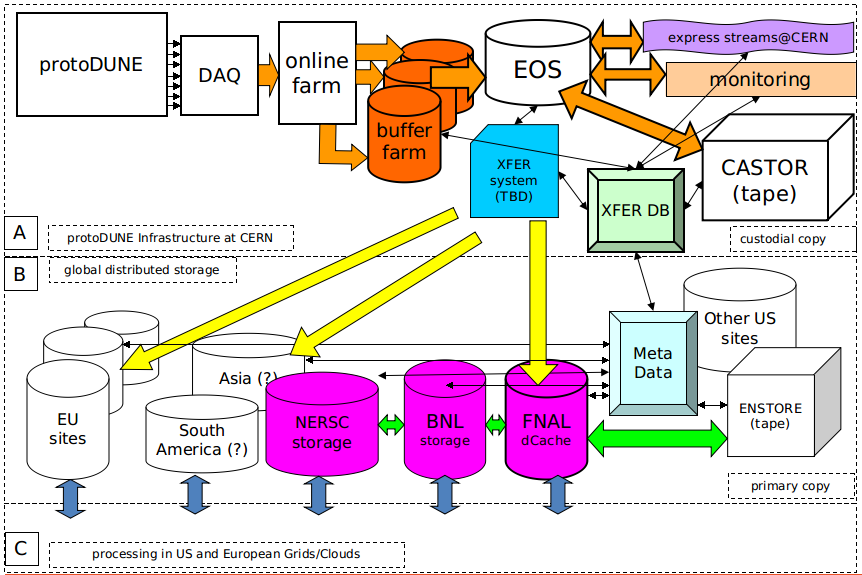
\includegraphics[width=\linewidth]{protoDUNE_raw_data_concept.png}
\caption{\label{fig:raw_concept}Conceptual diagram of the flow of raw data in \pd}
\end{figure}
%%%%%%%%%%%%%%%%%%%%%%%%

\noindent
Conceptual diagram of the raw data flow in \pd is presented in Fig.\ref{fig:raw_concept}. It reflects the central role of the EOS
system at CERN (the high-performance distributed disk storage) in the \pd raw data management scheme. This is motivated by the experience
and architecture of the LHC experiments. EOS serves as the staging area from which the data gets committed to archival tape storage at
CERN (CASTOR) and from which it is transmitted to a number of endpoints including principal data centers such as FNAL and others.
It is also used to provide input to QA and other express processing streams at CERN.

\subsection{Prioritization}

All of the many elements in the chain of data acquisition, storage, distribution and processing are critically important to derive physics results  from the data.
At the same time, certain components of the data chain need to be prioritized over others in order to reliably perform the measurements during a potentially
limited time period (depending on the SPS and LHC running schedule).

The priority components are the DAQ and the Raw Data Management System, which includes capturing the data coming out of the DAQ,
transporting the data to persistent mass storage and prompt Quality Assurance which is required to ensure corrective action can be taken
if the detector or certain system problems are identified in the QA process. The latter can be thought of as sophisticated monitoring done in near-time,
which implies a ``few minutes'' scale of processing.

\section{Requirements}
\subsection{DAQ Interface: buffering requirements}
\label{sec:daq_interface}
The plan is to have sufficient buffering capability in the DAQ for both NP02 and NP04. In this case, ``sufficient''
primarily means conforming to the CERN requirement that the experiment must be able to keep taking data for a
least 3 days at the nominal data rate, even if there is an occasional problem with the data link between the
experiment site and CERN central storage facilities, or an issue with the central storage systems or any type of similar outage.
At the time of writing, there are differences in how the two \pd experiments approach this:
\begin{itemize}
\item Buffer depth in NP02 is larger, in order to make possible some processing right in the data room of the experiment. A number of middleware options are being explored for this storage solution, in particular the BeeGFS file system.

\item In NP04 the emphasis is made on a more lightweight and fault tolerant setup which satisfies the general buffering and throughput requirements.
No extensive processing is foreseen on the experiment site. Among the possible technical options for the buffer farm file access is xrootd.
\end{itemize}
It is this ``outer layer'' of the data acquisition system (the buffer) in either experiment that will need to be interfaced with
the \pd raw data management complex.  It is represented as the block labeled ``buffer farm'' in Fig.\ref{fig:raw_concept}.

\subsection{Functional Requirements for Data Management}

The following is a summary of basic requirements for the \pd data management system:
\begin{itemize}

\item Transfer raw data files from both NP02 and NP04 online disk buffer farms
to CERN EOS disk and from there to CERN tape (CASTOR), FNAL tape (Enstore) and other end-points.

\item Ensure that the throughput is adequate and there are no bottlenecks for the Data Acquisition System
given the expected data rates over the nominal two month running% (see table)

\item Record file metadata inculding the file status and outcome of file operations

\item Operate at CERN and FNAL with support for initial setup and ongoing operations

\item Provide monitoring of overall system health, detection of error conditions and corresponding alerts, and support of troubleshooting

\item Provide triggers to perform file operations (copy, delete) based on configurable rules

\item Support ``express lane'' process at CERN and other institutions

\end{itemize}

\noindent
Table~\ref{fig:det_perf} contains performance measures driven by the expected extreme rates of each \pd detector
and which the file handling system must accommodate on the assumption that they apply to both detectors.


\begin{table}[tbh]
\centering
\begin{tabular}{l l l}
\hline
\textbf{Performance Benchmark} & \textbf{Single Phase} & \textbf{Dual Phase}\\
\hline
\hline
Raw data volume (total)                    & 1.2\,PB & 2.5\,PB \\
Raw data files (total)                      & 0.6\,M  & 1.2\,M\\
Avg. Data Rate                                & 20\,Gbps & 20\,Gbps \\
Latency to reach EOS                     & 10\,min & 10\,min\\
Latency to reach express lane processing & 10\,min & 10\,min\\
\hline
\end{tabular}
\caption{\label{fig:det_perf}Expected protoDUNE performance characteristics.}
\end{table}


% The file handling system assumes the following limits will not be exceeded (Table~\ref{fig:dh_perf})
%\begin{table}[tbh]
%\centering
%\begin{tabular}{l l l}
%\hline
%\textbf{Performance Benchmark} & \textbf{Single Phase} & \textbf{Dual Phase}\\
%\hline
%\hline
%Pending files in FTS dropbox             & 1~PB        & \\
%Simultaneous active files in transfer    & 50,000      & \\
%File registrations rate                  & 3600/hr     & \\
%File registrations                       & 200,000/day & \\
%\hline
%\end{tabular}
%\caption{\label{fig:dh_perf}Performance requirements for the data handling system used in the \pd experiment.}
%\end{table}

\section{General Design of the System}
\subsection{F-FTS}
The design presented here leverages the technology of the Fermilab File Transfer Service (F-FTS), which has been succefully applied
in a number of Intensity Frontier Experiments and demonstrated a high degree of robustness along with automation, integrated metadata
and extensive monitoring capabilities. In the following, instances of this system (run with different configurations) will be referred to
as ``FTS'' for brevity.

\subsection{FTS instances}
The baseline design for the online data handling system is shown schematically in Fig.~\ref{fig:sys_topology}.
The central idea of this design is a tandem of two FTS instances run as two separate systems within the CERN
computing environment, and interface each other. They will be referred to as ``primary'' and ``secondary'' FTS.
This does not reflect on their scale, prioritization or importance, but rather on their position in the data transmission chain.

\subsection{Primary FTS}
For both NP02 and NP04 the primary FTS system are deployed within or straddling the border
of each of the detector’s DAQ domains.

 and is configured to run on a system which is able to access the DAQ buffer disks either through a POSIX filesystem or
a protocol layer (e.g. xrootd, gridFTP or others).  The primary FTS system is configured on this system
to look at one or more input directories or storage locations, commonly referred to as a ``dropboxes''.
The FTS daemon performs periodic scans of the configured dropboxes. The system will operate asynchronously
and independently of the \pd DAQ systems.  When the \pd DAQ has produced a file that needs to be handed over
to the storage system, it will ``move'' (perform a filesystem/storage system atomic move operation or the equivalent)
the file to the dropbox location. When a new file is located within one of the dropboxes,
the system will initiate the file registration and transfer operations.

%%%%%%%%%%%%%%%%%%%%%%%%
\begin{figure}[tbh]
\centering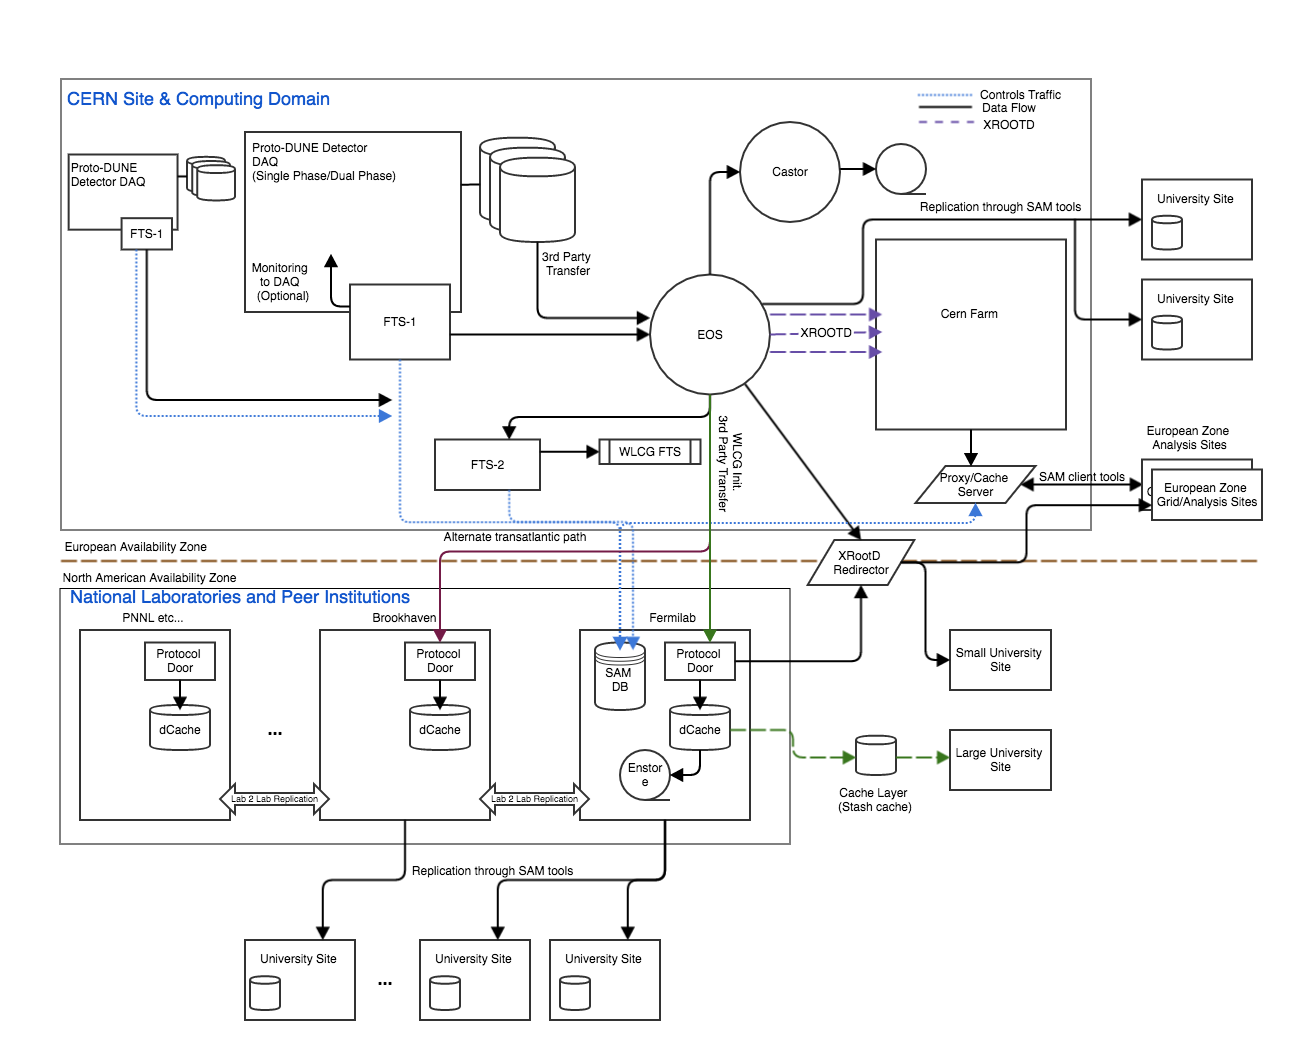
\includegraphics[width=0.99\linewidth]{protDune-datahandling-topology.png}
\caption{\label{fig:sys_topology}\pd data handling system topology}
\end{figure}
%%%%%%%%%%%%%%%%%%%%%%%%
In the \pd model, the primary F-FTS will initiate a copy operation from the online disk buffer farms into the EOS storage system. 
The system will use the 3rd party copy support that is provided by the xrootd protocol to allow for optimized transfers into EOS. 
Upon completion of the initial copy into EOS, the F-FTS will initiate a ``chained'' copy (a copy that is dependent on the initial copy into EOS)
of the data from EOS to the Castor archive system.  The F-FTS system will register each file’s metadata records (containing both basic and
physics metadata, defined below)  in the SAM data handling system.  Upon completion of the replication of the data to Castor,
the F-FTS will enter a monitoring/polling state of its operations to determine when the file has been successfully written to the archival media.

\subsection{Deletion and Cleanup}

%%%%%%%%%%%%%%%%%%%%%%%%
\begin{figure}[tbh]
\centering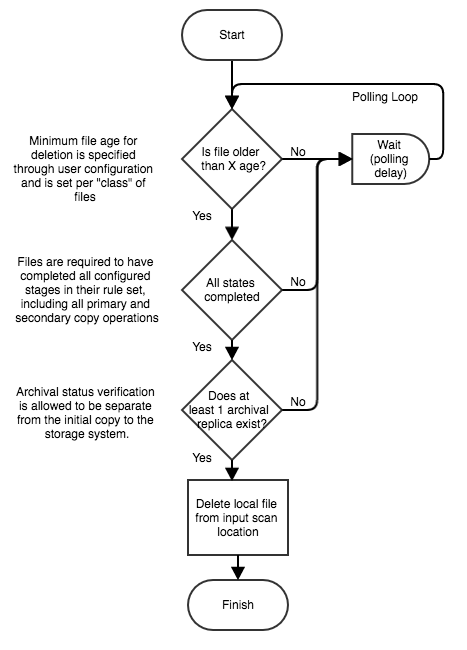
\includegraphics[width=0.5\linewidth]{fts_file_deletion_flowchart.png}
\caption{\label{fig:ftscleanup}Flowchart of the \pd file deletion and cleanup.}
\end{figure}
%%%%%%%%%%%%%%%%%%%%%%%%
The primary F-FTS will handle the “cleanup” of its input dropbox,
with configurable periodic cleanup passes through its current file sets.  Basic logic of the cleanup process is shown in Fig.\ref{fig:ftscleanup}.
Central to this is a configurable multi-stage validation procedure to determine if files are eligible for deletion/cleanup from the input area.
In particular the system can verify the archival status of files (ensuring they have been written to tape and that tape has been closed/unloaded properly)
prior to performing any file deletion.

The system may also provide an ``age'' criterion on files so that files can be retained within the DAQ environment for a specific period of time.
This allows operations like online/nearline processing or log files to be examined within the DAQ environment after the actual transfers to archival
storage have completed.



\subsection{Secondary FTS}
This secondary FTS system is configured to monitor the EOS locations that the primary FTS system is using as its output endpoint.
These EOS areas serve as the input dropboxes for the secondary system. It operates in the same manner as the primary FTS,
scanning for new files and then initiating copy requests of the data to a set of one or more destination endpoints.

%This F-FTS system will initiate the copy request between the European availability zone, and the North American availability zone.  

At least one of the endpoint destinations for this service will be the FNAL-based dCache/Enstore system, where a second archival
copy of the data will be recorded.  Additional copies to participating sites can be
configured based on available resources and available bandwidth (e.g. direct transfer from CERN to BNL’s dCache or to PNNL’s storage facilities). 
To perform the transfers, the F-FTS will interface with the WLCG-FTS (as a supported transfer protocol) to schedule the actual transfer
between the storage elements.  

The exact locations of the endpoints and corresponding policies will be determined at a later date. For more comments on data replication
please see \ref{sec:replication}.


\subsection{Data Catalog}
Underlying the F-FTS systems will be a fully featured data management layer (SAM) which will provide the metadata and replica catalogs.
All data being handled by the transfer systems will have corresponding records in the data handling catalog so that the content,
locations and provenance of the data can be fully tracked.  The primary catalog systems will reside at FNAL with proxy/cache
layers in the European and North American zones to ensure high speed connections between the servers and the (offline analysis)
clients that will query the catalogs from these zones.  Similar scalable proxy and cache layers can be instantiated for other identified
zones which may require high speed or optimized access to the catalog systems.
 
\subsection{Replication}
Replication between collaborating peer institutions in the same geographic zone  (e.g. national laboratories and large universities with significant
computing/storage resources in the North American zone) will be provided through standard ``dataset'' replication tools that are a part
of the SAM data handling suite.

Data access at smaller university sites or opportunistic computing resources (e.g. Open Science Grid
affiliated sites) is provided and optimized through support for streaming protocols such as xrootd with redirector
services and through cache layers such as the “stash cache” system employed by the Open Science Grid.  

\section{Technical Requirements to the FTS Components}

\subsection{Outage and Backlog Considerations}
\label{sec:backlog}
As already mentioned in Sec.\ref{sec:daq_interface},
CERN policies require that an experiment is capable of storing data locally (in the vicinity of the apparatus as opposed to CERN Central
Storage)  for a nominal period of 3 days, to ensure that the experiment can run for a period of time even in case of network interruptions
and storage facility outages.

In an outage scenario the data preserved locally must still be committed to mass storage when a service is restored.
This creates a backlog situation which roughly doubles the requirements on the sustained rate of file registration and other transactions, buffer
areas and certain other parameters of the overall system. This will be reflected in some of the numbers presented below.


\subsection{Data Throughput}

The data management system must perform in a way that allows for full exploitation of the underlying hardware and networking infrastructure
upon which  it is running.  In the case of the \pd experiments the FTS system will be capable of operating at a sustained data processing and transfer
rate that is greater than 80\% of the maximum theoretical bandwidth available between the DAQ buffer farms and the EOS storage system.
In the current design this network bandwidth consists of two 20\,Gb/s ethernet links.
%  The RAID arrays or distributed file system architectures to which the data will be written to and read from are assumed
% to have similar or lower available bandwidth.
This sets the upper limit of the throughput of the entire system, with other components operating at this or perhaps lower levels.
The actual observed read/write bandwidth will be determined by configuration of the detectors and the combination
of the DAQ hardware and software.


  The primary DAQ FTS system will be required to operate at a sustained effective bandwidth
of the lesser of: two times 16\,Gb/s (80\% of theoretical network bandwidth) or 80\% of the measured read access bandwidth from the storage arrays
of the buffer farms
(during simultaneous write operations, if the DAQ computing models requires this mixed access mode) under the standard \pd operations.

\subsection{Transaction Throughput}

In terms of transaction handling,  the data management system must be capable of fully leveraging the data
catalog and infrastructure in order to meet or exceed the rate at which files or other data
objects are generated by the \pd detectors amd their DAQ components.

Given the nominal file size of 2\,GB (used here purely for estimation purposes), 
the primary FTS system mist be able to support a minimum transaction rate of up to 1\,s$^{-1}$
and the corresponding aggregated total of $\sim$10$^5$ file registration operations per day.
This level of performance has been demonstrated in other deployments of this type of data
handling system.

\subsection{Transaction Tracking}
The data management system must be able to perform simultaneous end-to-end tracking
of all files that are in state of transit the system prior to being written/verified in the archival storage,
without impacting or interrupting data taking.  To achieve this goal the transaction tracking system for \pd will be
able to support a total number of ``in flight'' files per FTS instance equal to the nominal number of transactions per day
(estimated above as $\sim$10$^5$) times the maximum supported duration (in days)
of an outage that can be sustained by the DAQ system under outages in the downstream network or storage domain.
As mentioned above, such duration is defined as 3 days per the CERN policies. In addition, due to data backlog considerations
(see \ref{sec:backlog}) there must be another factor of 2 added to guarantee transport of all data to its destination during
the recovery period.

In summary, the FTS systems will support at least 6$\times$10$^5$ files in state of transit at any given time,
where at least 10$^4$ of these files are undergoing ``active'' registration/transport through the system at any given time.
In other words, $\sim$10\,k of the files are being actively
managed and their status is constantly updated while the remainder are “waiting” in the designated dropbox location.

\subsection{Transfer Latency}
The file transfer and management systems are designed to operate in an asynchronous manner to other components of the \pd DAQ. 
Due to the polling models employed in this asynchronous model, many operations do not have fixed temporal relations to other events in the DAQ system,
but rather will occur/complete within a well defined time window or with a certain latency.  In the case of the \pd experiment,
the data management systems will be capable of operating as detailed below.

In the primary FTS, the latency between the completion of the DAQ writing a file and the hand-off/detection of the file by the
system will be controlled by a configurable delay parameter (in minutes) which defines the polling intervals for the FTS
to look for ``new'' files in its input dropbox locations.  Under normal (steady state) operation, the average latency will be 1-2 polling intervals.
The actual latency may be bigger depending on the number of other new or pending files currently in the system.
In this case the order of file handling will be managed by an internal queuing algorithm that efficiently operates on the files but
does provide any user specified prioritization.

In the second stage of file transfers, the latency between when a file is generated by the DAQ and when it is transferred to the EOS
system and then written/verified to archival media (via CASTOR) is dependent on first stage latencies (new file detection and file registration)
and then the details of the archival storage system and its characteristics.  In particular the DAQ to EOS to CASTOR path will constitute a set
of chained dependencies with an independent polling interval for each stage.  Under normal operating conditions that latency for the file to
be transferred to EOS and be available through the data handling system is expected to be 1-2 of these polling cycles, contingent on write
congestion in the EOS storage system.   For full registration of the files in Castor and onto type, the FTS/SAM systems will support latencies
in this recording of 3 hours to 30 days and will support a configurable timeout parameter to indicate failures in this transition.

The latency between when files are written by the DAQ and when the files are available on storage in the North American zone,
will be determined by the second stage latency of the files appearing on the EOS system from the DAQ and then a secondary latency
will be incurred based on the polling for files that require transatlantic endpoints.  Similar to the other stages this is configurable
through a polling interval.  Once queued for handling the actual file transport will be off loaded to the WLCG FTS system which will
schedule the files for transmission and will properly balance and throttle the site to site traffic and will properly conform to the CER
 computing environment.  Latencies at this stage are well understood based on the experience that the LHC experiments have with WLCG FTS.  

\section{Data Management System Interfaces}
\subsection{Overview}
The modular design of the data handling system will provide considerable flexibility in its ability to adapt to different requirements
for interfacing  both data input and output systems.  In the \pd experiment the most important interfaces are to be established with
\begin{itemize}
\item the experiment’s core DAQ components
\item mass storage and data archival at CERN
\item mass storage and data archival at FNAL
\end{itemize}

\noindent
 Details of these interfaces are presented below.

\subsection{The DAQ Interface}
The interface between the core DAQ system and the data handling system is made at the DAQ’s disk buffer farm.
When the final stage event builder have completed the assembly of a file, the file will be handed off to the data handling system
by the DAQ by placing the file into a designated ``dropbox'' area on the target file system.  For POSIX compliant file systems,
this can be accomplished through an atomic move operation (i.e. Unix \textit{mv} equivalent) which minimizes the I/O overhead associated
with the hand off.  No signals need be emitted from the DAQ, nor will any other form of message be required in the direction of the
DAQ to the data handling system.  The F-FTS will detect new files through files becoming visible in configured dropbox locations of
the storage system (i.e. a new file appearing in a directory) 

The F-FTS systems running as part of the data handling system will use either a POSIX (or near POSIX) compliant file system view of the disk buffer farm,
or an API that provides access to standard meta information regarding the storage system’s dropbox area (directory) and contents
(i.e. filenames, file size, create/modify times etc…)  Additionally the FTS will require a file read API for the purpose of metadata
extraction from the file and for checksum computations (if not provided through some other means).  The system will require a
delete API and privilege, if the automated cleanup options are desired/enabled.  If the DAQ storage elements support ``third party''
transfer protocols, the FTS can use these to reduced overhead in performing the actual file transfer operations.

The organization of the FTS dropbox area(s) will be configured to support the volume of data that would be generated during a
sustained outage (of non-DAQ systems) of no less than 3 days plus the time required to register/process the volume of data
that would be generated during the outage (i.e. ``the recovery time'' required to clear a backlog).

\subsection{The EOS Interface}
The interface between the data handling system and the EOS storage system will be made through the APIs
provided by the standard protocols already supported by both the EOS system and the SAM data handling system.
In particular the xrootd protocol will be the primary API used for the interaction between the system, with secondary
support for the gridftp, webdav and srm protocol APIs.  The EOS system will be declared, and configured in the SAM
system as a standard storage element and will have files stored on it registered and mapped within SAM the replica
catalog to the well defined access URIs. 

\subsection{The CASTOR Interface}
The interface between the data handling system and the CASTOR archival storage system for file ingest will be made through the
APIs provided by the standard protocols already supported by both the CASTOR system and the SAM data handling system.
In particular these system both already support the xrootd protocol, gridftp and srm.  The CASTOR API to query the tape archive
interfaces (to determine if a file has been successfully archived to tape and which tape it is located on) will be integrated into the
SAM data handling system in a manner similar to other tape systems that SAM is already aware of (i.e. Enstore)   The CASTOR
system will be declared, and configured in the SAM system as a standard tape storage system and will have files stored on it
registered and mapped within SAM the replica catalog to the well defined access URIs along with additional tape location information
to permit optimized retrieval.  Custom modules/utilities will be developed as needed as part of the SAM data handling suite to provide
additional support for the CASTOR system in performing certain operations (i.e. bulk queries or monitoring operations).
These modules/utilities will be distributed as part of the core SAM distribution.

\subsection{The dCache/Enstore Interface}
The interface between the SAM data handling system and the dCache/Enstore archival storage system is already fully defined and supported.
 The interface fully supports standard access protocols including xrootd, gridftp, webdav and srm as well as the proprietary \textit{dcap} protocol
and a specialized NFS implementation that provides limited basic read access for hosts with local mounts of the dCache system.
The SAM system has modules that optimize data access based on Enstore tape location information.  This interface is in wide scale
production use across many experiments including NO$\nu$A, $\mu$BooNE, the DUNE 35t prototype, MINOS and others.

\subsection{The SAN/NAS Interface}
Generalized SAN and NAS systems when acting as data sources (input) will be integrated to the data handling system through their
POSIX style interface if available.  When enabled as data sinks (output) for the data handling system, a front end data server(s)
running standard access protocols in the form of xrootd or gridftp will be utilized.  These will then be mapped into SAM as standard storage locations.
  
\subsection{Generalized Protocol Support Interfaces}
The data handling system provides a file delivery and transfer layer which acts to provide protocol abstraction to the end users
(i.e. provides a consistent command interface) and provides a protocol bridge when performing transfer operations between dissimilar
storage systems (i.e. cross protocol transfers).  The ``Intensity Frontier Data Handling'' tool (IFHD) for \pd will support protocol integration for:
\begin{description}
\item[XROOTD] Full support will be provided for xrootd in the Fermi-SAM data catalog, F-FTS and IFDH layers.  Currently these tools support read/write access methods.  Full support for additional xrootd features (listings, permissions modification, etc...) is currently under development.
\item[WLCG FTS] SAM, F-FTS and IFDH will support WLCG-FTS as a 3rd party or proxy transfer mechanism.  In this mode outbound file transfers originated from the CERN domain can offloaded to WLCG-FTS so that the data traffic across the CERN site can be properly scheduled and balanced.  Support for this mode of operation will be integrated into IDFH or directly into the sam\_cp layer of the F-FTS. 
\item[GridFTP] This protocol is fully supported for most of the components involved, but is not the preferred or documented interface for any of the CERN storage components.
\item[SRM] This protocol is fully supported for most of the component systems involved, but is not the preferred or documented interface specification for the CERN storage components.
\item[HTTP] Fermi-SAM uses HTTP for internal communication between Fermi-FTS and the Fermi-SAM instances, and for client programs wanting file location and metadata information. It is also a supported file transfer interface into DCache.
\item[CVMFS] The data handling suite includes support for distributing its client tools and homing other parts of the suite on a CVMFS read-only filesystem.  This support allows the experiments to provide widespread, efficient code distribution over a HTTP based protocol while providing a file-system layer to the end user applications.  This is a standard distribution method used to to distribute the DUNE and LARSOFT software, as well as Fermi-SAM client utilities. 
\end{description}

\section{Data Replication, Registration and Catalogs}
\subsection{Replication}
\label{sec:replication}
The data handling system must be able to manipulate multiple replicas of the data across storage systems and locations, in order
to optimally utilize computing resources for production purposes, and make processed data readily available to researchers in
a number of geographical areas.
%It will be necessary to replicate data files or data sets between sites or storage locations. 
The data handling systems for \pd will handle this replication in different ways
depending on geographic proximity and bandwidth.  At least two ``Primary Zones'' can be identified in order
to describe data locality in \pd -- the \textit{European Zone} and the \textit{North American Zone}.

The European Zone encompasses CERN and other institutions near to CERN geographically and in network bandwidth proximity,
while the North American zone would includes  FNAL, BNL, the other institutions
in close network proximity to the major member institutions of the DUNE collaboration which are located in the US.
Replication within the primary zones will be handled in the following manners by the data handling system:

\begin{description}
\item[European Zone] -- Replication and data transfers within the CERN domain will be handled by F-FTS instances configured with site specific endpoints rules (i.e. the EOS and CASTOR rule sets) which will provide for the full data sets to available in both EOS and CASTOR.  Transfer and replication operations outside the CERN domain to institutions with registered storage elements will be performed through the SAM suite’s replication tools (sam\_clone\_dataset).  Transfer or replications to smaller institutions or analysis sites without registered storage elements can be performed through the SAM/ifdh client tools (ifdh\_fetch).  The SAM client tools are which are available through CVMFS.  

\item[North American Zone] -- Initial replication of the data to FNAL, BNL and other collaborating labs or large university sites will be
automated through F-FTS instances at CERN and in North America which will be used to optimize the data transfer paths to each of
the institutions, subject to bandwidth constraints of the host institutions.   Transfers elsewhere in the North American side would be
performed using the same SAM tool suites and strategy for handling registered and unregistered storage, as specified above for the European zone. 

\item[Other Institutions] -- Organizations wishing to host a set of datasets or partial data sets will be able to register their storage
elements with the SAM data catalog and will then be able to use the replication tools to clone the relevant data to their site. 
\end{description}

\subsection{File Registration}

Registering files or other forms of data with the SAM catalog require a set of “meta information” about the files.  This information is used to allow detailed searches to be performed to select specific data for analysis.  This metadata is broken into two general types “Base Metadata” and “Physics Metadata” which can be provided at the time of file registration, or modified later.  These metadata are composed of:
\begin{itemize}
\item Base Metadata -- For each file the the Fermi-SAM database requires a unique filename, the file size, and a file type string. It also allows one or more checksums - each consisting of an algorithm type name and a value - and a description of the application used to create the file. The file can also have zero or more parents (which much be files already existing in the catalog) which creates a tree of relationships between files.
\item Physics Metadata -- There are a number of predefined physics metadata fields such as the detector configuration, the run number, the data tier, the event count, the start time and end time, and the data stream. It is also possible to define arbitrary key names for other values with either integer, float (64 bit), or string types.
\end{itemize}

The experiment must provide a method for determining or generating the metadata (i.e. an external program that can be run on a file, or a python module that extracts information from a filename, etc…)  and that method will be invoked by the data handling system when it encounters appropriate files.  The output of the method used must conform to a suitable format supported by the F-FTS and SAM systems.  The systems support JSON formatted files and python dictionaries for direct upload to the data catalogs.  

\subsection{Data and Replica Catalogs}

The data management system for \pd will leverage the DUNE experiment’s SAM data catalog.  The underlying resources of this catalog and its software are capable of, and sized to support, a file inventory in excess of 150 million files (demonstrated by the DØ experiment’s catalog which uses the same technology).  The data catalog provides a command line toolset for both client and administrative functions, as well as a web based API for interacting with the catalog.  The web tools provide additional guidance for assisting users in finding and classifying data through the indexes.

The data management system will also leverage the same DUNE instance of the SAM catalog to maintain its replica catalog.  This instance will provide a unique namespace for the DUNE/\pd experiments and will contain the appropriate storage identifiers and paths to enumerate the full locations of  DUNE/\pd data on all supported sites.  The SAM replica catalog itself is protocol neutral, but a mapping layer within the data handling system performs the translation of locations into actual access URLs of the default, preferred or requested protocol schema for a given storage system (i.e. the system maps the location onto the method for how you retrieve the file).

\section{Data Transfer Technology}

The data management system for \pd will support, through its use the SAM tool suite,  data transfers to and from CERN, FNAL and other site’s storage elements using a combination of protocols supported by the specific site’s storage resources.  In particular the system will natively support the xrootd, gsiftp (gridftp), webdav(http), and srm protocols for access to EOS, Castor and dCache/Enstore (as appropriate).  The system can support multi-channel transfers and 3rd party transfers using these protocols to achieve high bandwidth or low overhead transfers where needed.  The system also supports operations specific to local access methods on POSIX file systems.  

The file transport layer uses a modular design with an abstraction layer so that new protocols or access methods can be added to the system without changes to the other interface layers.  The system can also select or prioritize the replica source location and access protocol based on destination characteristics (i.e. it can prefer a local cache copy of a file to a replica that is at a transatlantic location)  The system will also support offloading of transfers to 3rd party transport systems (e.g. WLCG FTS) to properly balance the resources of different WAN connections and site resources.



\end{document}
